\section*{第四章~~暗物质探测实验现状}

\setcounter{section}{4} \setcounter{subsection}{0}
\setcounter{table}{0} \setcounter{figure}{0} \setcounter{equation}{0}

\addcontentsline{toc}{section}{第四章~~暗物质探测实验现状}

暗物质的探测手段可以分为直接探测实验和间接探测实验。直接探测实验,即通过探测暗物质粒子与实验靶核子的散射来确定暗物质的存在;间接探测实验,即探测暗物质湮灭或衰变产生的各种粒子,从而确定暗物质的存在。

\subsection{直接探测实验}

直接探测的基本思想是:若暗物质粒子(如 WIMP)穿过地球时与原子核发生弹性散射,可在地下探测器中留下微弱信号。由于背景噪声(如宇宙射线、天然放射性)极高,因此这些实验通常建在深地下实验室中,以屏蔽干扰。

\subsubsection{DAMA 实验组}

银河系被认为由一个均匀分布的暗物质晕(halo)包围,暗物质粒子在其中随机热运动。太阳系绕银河中心公转的速度约为 220 km/s,形成了一个“暗物质风”。地球则绕太阳公转,速度约为 30 km/s。

地球在 每年6月的运动方向与太阳运动方向一致,与“暗物质风”相对速度最大。在 每年12月,两者方向相反,与“暗物质风”相对速度最小。暗物质粒子与探测器中原子核的弹性散射率和能量沉积随速度变化,从而导致探测率呈现一年周期的调制。DAMA 使用 高纯度碘化钠闪烁晶体(NaI(Tl)) 作为探测器,监测中低能核反冲事件的计数率。数据处理过程中排除日常背景变化和伽马射线等非WIMP事件的影响,关注随时间变化的微弱周期信号。

\begin{figure}[!htbp]
    \centering    
    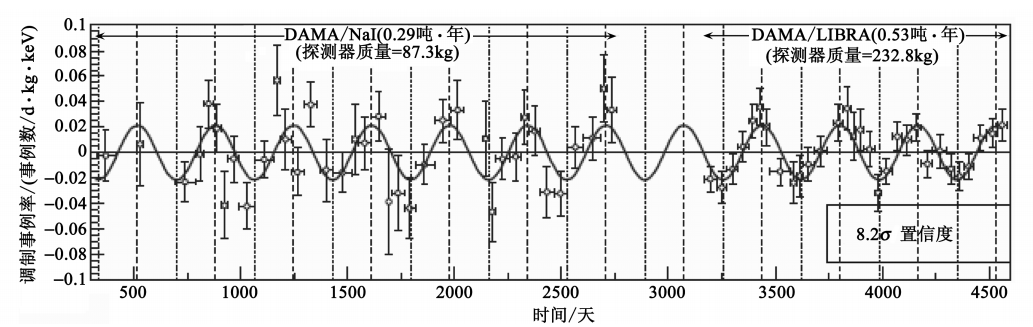
\includegraphics[height=5cm]{Img/4-1.png}
    \caption{DAMA 实验观测到的年调制信号.这有可能是来自于暗物质碰撞的信号 }
    \label{4-1}
\end{figure}

然而,除了 DAMA 实验组外,其他实验组均未看到暗物质碰撞的正面信号,暗物质的信号至今还未被其他实验所证实。

\subsection{间接探测实验}

间接探测的目标是寻找暗物质湮灭或衰变产生的产物,如高能 $\gamma$ 射线、反质子、正电子或中微子。这类信号通常来源于暗物质密度较高区域,如银河中心或星系团。

\subsubsection{PAMELA 实验组}

2008 年,欧洲的 PAMELA 卫星实验公布了宇宙线中反物质的探测结果,显示地球附近太空中的正电子能谱在能量约高于10GeV 的区域内明显上升,与传统的宇宙线理论预言的下降能谱不符合,同时该实验组在能量约低于100GeV 的能区内未探测到超出背景的反质子。

\begin{figure}[!htbp]
    \centering    
    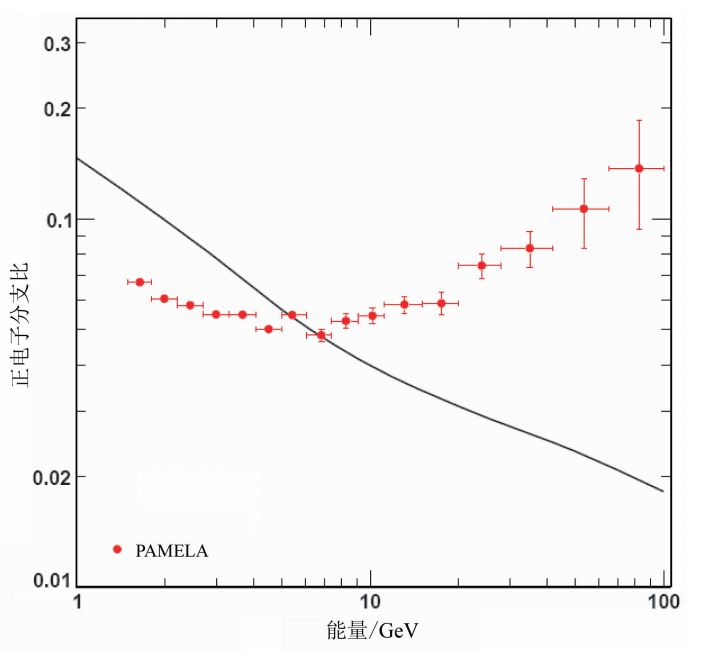
\includegraphics[height=5cm]{Img/4-2.png}
    \caption{PAMELA 卫星实验观测结果。实线对应理论背景预期结果,红点为实验观测数据。 }
    \label{4-2}
\end{figure}

很多研究者试图用暗物质来解释正电子的超出,但是为了避免反质子的超出,必须接受一个结果即暗物质的湮灭主要产生轻子对,而不是夸克对。这对传统的暗物质模型提出了挑战。

\subsubsection{ATIC 实验组}

ATIC 使用的是高空气球平台,飞行高度约为 35–40 km,能在大气层之上长时间运行(特别是在南极可以利用极夜形成的平流层气流循环,飞行时间达几周)。其主要目标是测量宇宙线中电子(包括正电子)通量与能谱。

\begin{figure}[!htbp]
    \centering    
    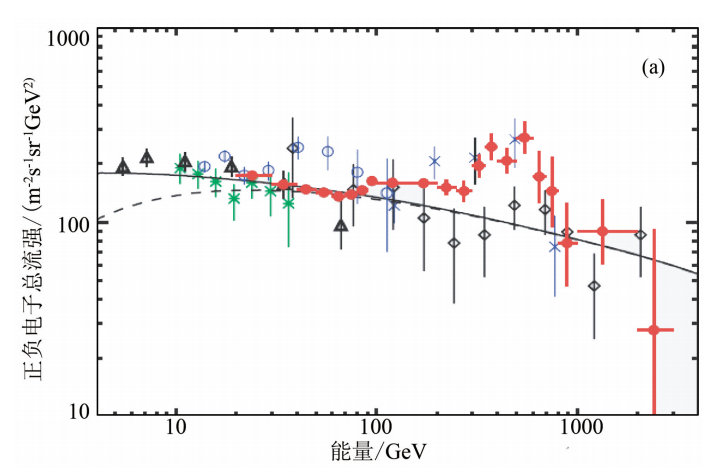
\includegraphics[height=5cm]{Img/4-3.png}
    \caption{ATIC 实验组2008年公布的正负电子流量的数据。红色数据点为 ATIC 在2008年公布的数据,其余数据点为之前实验测量数据;实线和虚线为不同理论模型给出的正负电子流量的背景预测值。 }
    \label{4-3}
\end{figure}

ATIC 实验组观测到正负电子流量之和在 300 GeV 到 800 GeV 有一个明显超出,并且能谱有明显鼓包结构。这种异常可能来源于暗物质。

\newpage